\documentclass{PoS}

\usepackage{ptdr-definitions}

\providecommand{\NLOJETPP} {{\textsc{NLOJet++}}\xspace} \providecommand{\kts}{\ensuremath{k_{\mathrm{t}}}\xspace}

\title{Jet and photon physics in pp collisions at the LHC}

\ShortTitle{Jet and photon physics in pp collisions at the LHC}

\author{\speaker{ Vitaliano Ciulli }% %\thanks{} \\ Dipartimento di Fisica, Universit\`a di Firenze and Istituto
Nazionale di Fisica Nucleare, Sezione di Firenze, via G. Sansone 1, 50019 Sesto Fiorentino, Italy \\ E-mail:
\email{vitaliano.ciulli@fi.infn.it}} \author{on behalf of the ALICE, ATLAS, CMS and LHCb collaborations}

\abstract{}

\FullConference{Fourth Annual Large Hadron Collider Physics\\ 13-18 June 2016\\ Lund, Sweden}

\begin{document}

\section{Introduction}

Quantum chromodynamics (QCD) is the fundamental theory describing strong interactions among partons, \ie quarks and
gluons. Jets and photons production at the Large Hadron Collider (LHC) at CERN are key processes to test predictions of
perturbative QCD (pQCD) over a wide region in phase space. They are also among the main backgrounds to new physics
searches and therefore needs to be measured with the highest possible precision to allow discovering the tinest
deviations between data and theory.

The LHC collaborations, ALICE~, ATLAS~\cite{Aad:2008zzm}, CMS~\cite{Chatrchyan:2008aa} and LHCb, performed
measurements of inclusive jet production, multi-jets production, jet properties and photon and diphoton production. 
In the following we will review most recent measurements.

\section{Jet Physics}

Jets are usually reconstructed with the anti-\kts algorithm~\cite{Cacciari:2008gp} with different values for the distance parameter $R$.
ATLAS uses topological clusters~\cite{Lampl:2008zz} of cells in the calorimeter as input objects. 
In CMS and LHCb, the particle-flow (PF) event algorithm~\cite{CMS:2009nxa}
first reconstructs and identifies each individual particle with an optimised
combination of information from the various elements of the detector. Next PF objects are used as input to the jet
reconstruction algorithm. ALICE uses both tracks and energy deposits in the
Electromagnetic Calorimeter to reconstruct jets in the region $|\eta|<0.9$.

The main experimental difficulties are the jet energy calibration and resolution estimate and the subtraction of pileup
effects. Additional proton-proton interactions (pileup) produce unwanted calorimetric energy depositions and additional
tracks. Different strategies have been developed to subtract these effect depending on the jet recontruction.
Furthermore, to compare with measurements, the parton-level calculations must be complemented with corrections for nonperturbative
(NP) effects that involve the modeling of hadronisation (HAD) and multiparton interactions (MPI).

Inclusive jet production measurements have been perfomed with data collected at different centre-of-mass energies, ranging from 2.76 GeV to 13 TeV. 
Using 13 TeV data collected in 2015, the CMS experiment measured the double-differential inclusive jet
cross section as a function of the jet \pt and absolute jet rapidity $|y|$.\cite{Khachatryan:2016wdh}. The data samples correspond to
an integrated luminosity of 71\pbinv. During data collection the LHC operated with a $50\unit{ns}$ bunch spacing and the
average number of pileup interactions observed in these data is ${\approx}19$. 
%The results are compared to fixed-order
%predictions at NLO precision, complemented with electroweak and nonperturbative corrections, and to predictions of
%various Monte Carlo (MC) event generators that combine leading-order (LO) or NLO pQCD with the modeling of parton
%showers (PS), HAD, and MPI.  

Figure~\ref{fig:crossSection} shows the double-differential inclusive jet cross section measurements,
presented as a function of \pt for seven $|y|$ ranges, after
unfolding for detector effects, using the anti-\kts algorithm with $R =
0.7$ and $0.4$, respectively. The measurements are compared to the predictions from \POWHEG +
\PYTHIA. The data are remarkably consistent with the predictions over a wide range of jet \pt from 114\GeV up to
2\TeV.

\begin{figure*}[htbp] \centering
  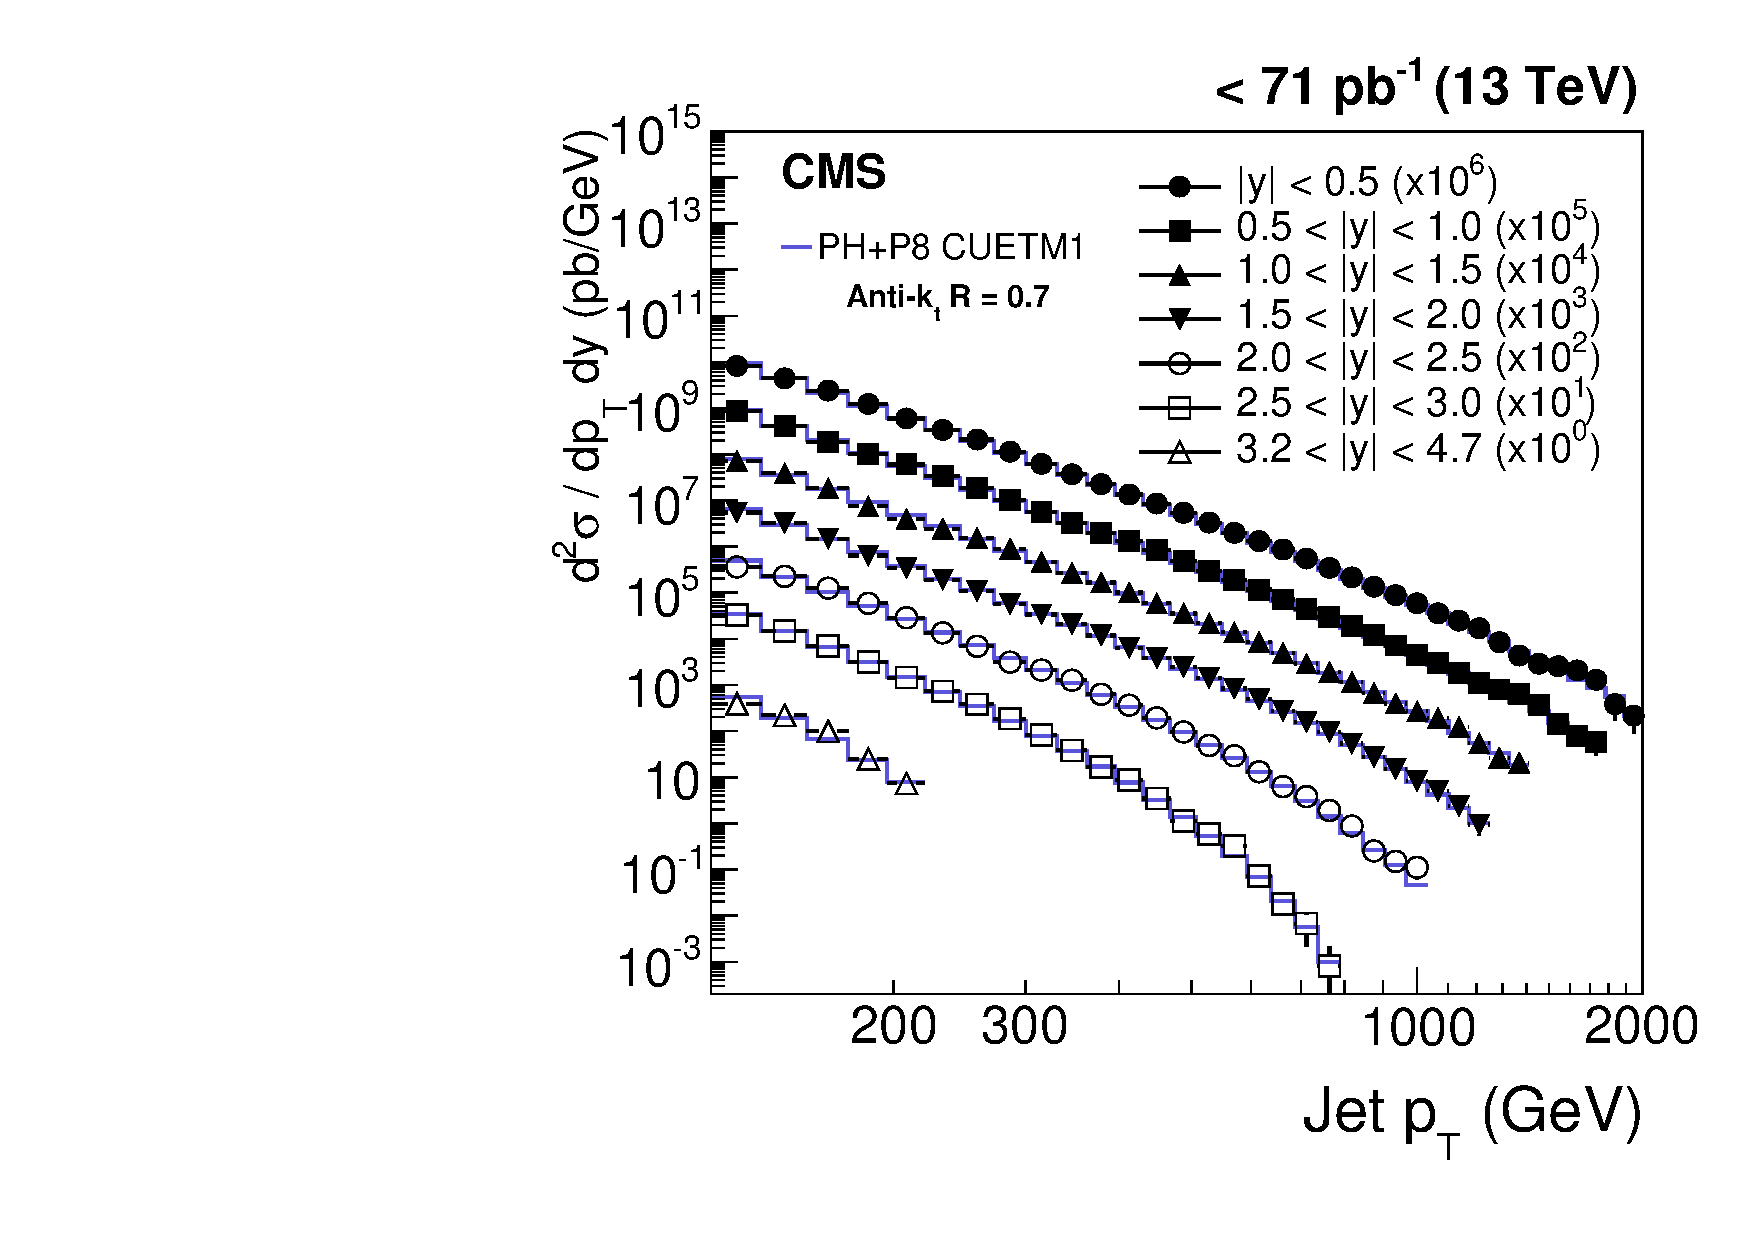
\includegraphics[width=0.48\textwidth]{Figure1-a.pdf}
  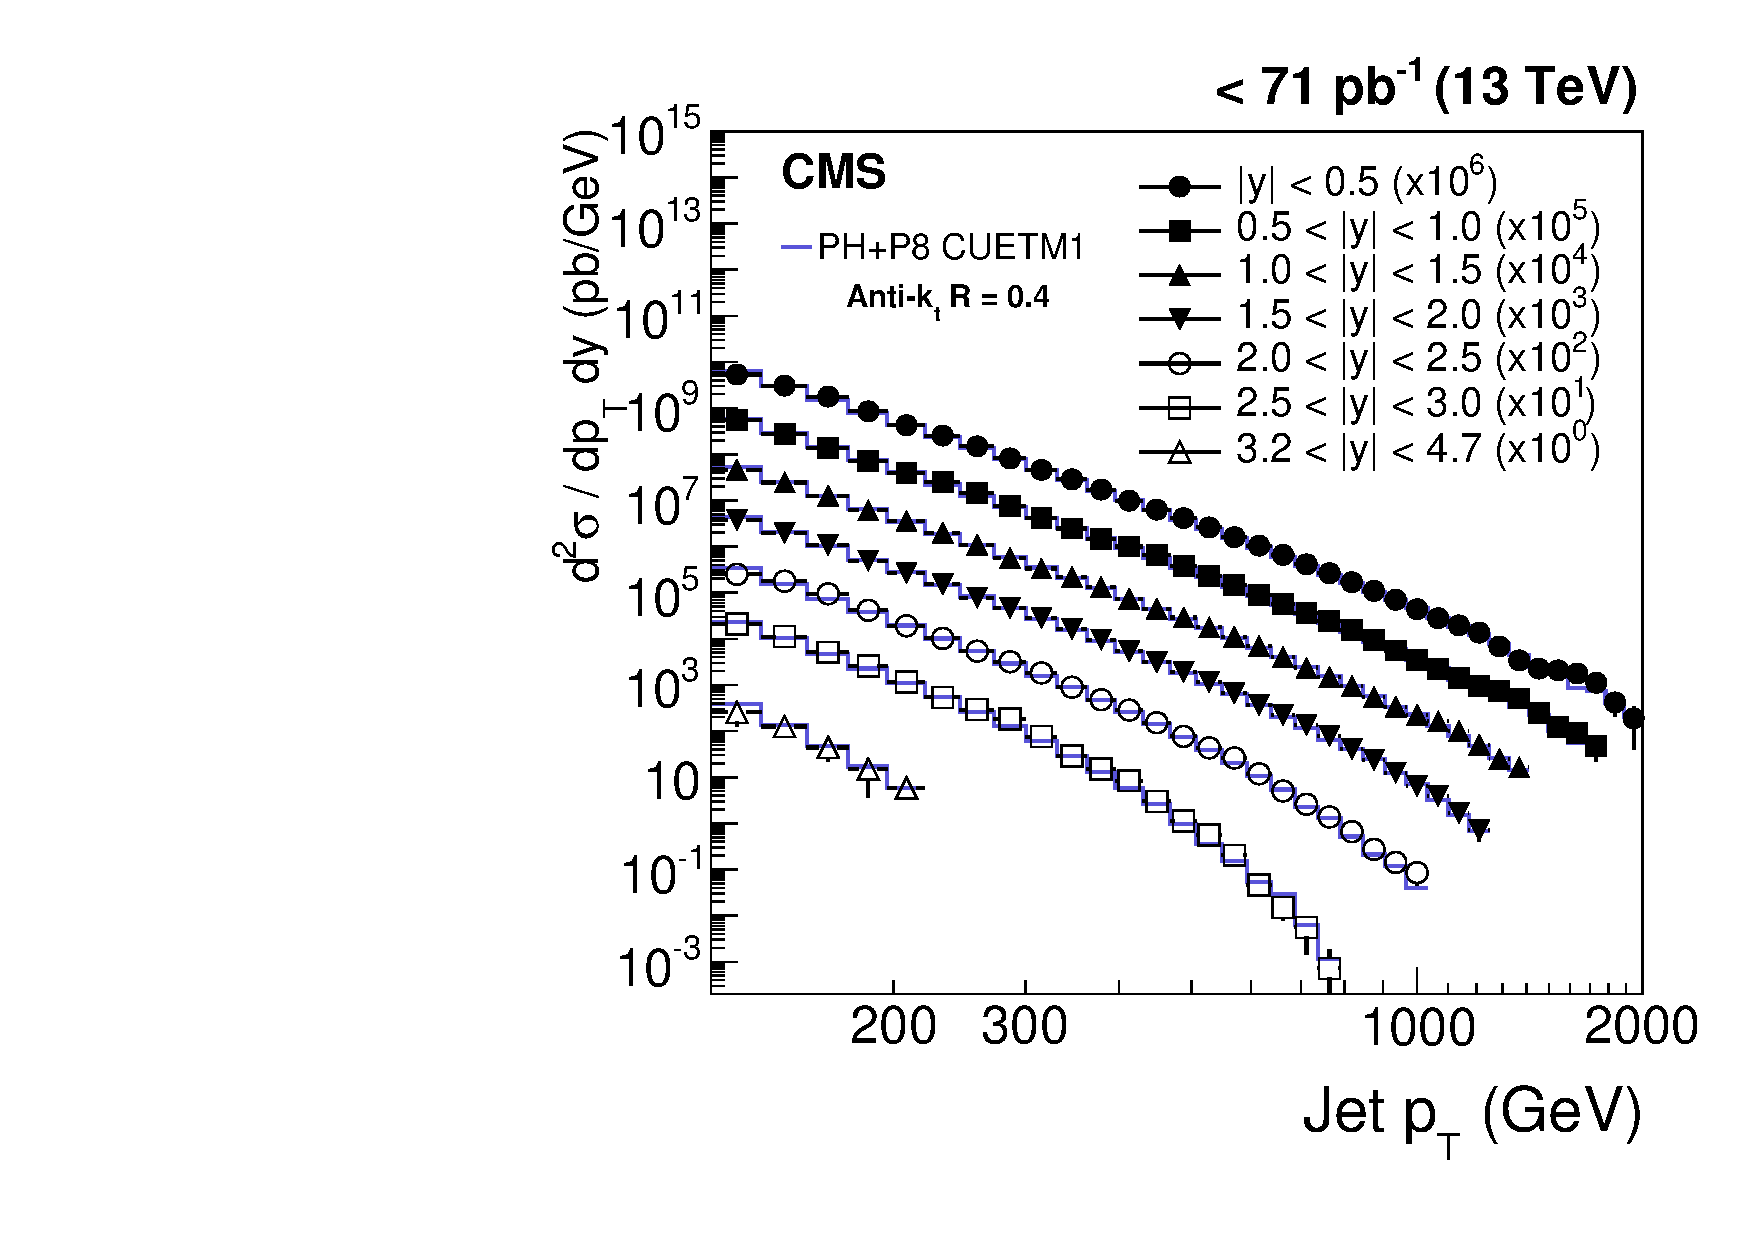
\includegraphics[width=0.48\textwidth]{Figure1-b.pdf}
  \caption{Double-differential inclusive jet cross section as function of jet \pt at 13 TeV. Data (points) and
predictions from \POWHEG (PH) + \PYTHIA (P8) with tune CUETM1 (line) are shown. Jets are clustered with the anti-\kts
algorithm with $R = 0.7$ (left) and $0.4$ (rigth).}
  \label{fig:crossSection}
\end{figure*}

The measurements are also compared to the \NLOJETPP~\cite{Nagy:2003tz} predictions using the CT14 PDF set~\cite{Dulat:2015mca}, corrected for NP and electroweak effects.
The ratios of data over the \NLOJETPP predictions are shown in Fig.~\ref{fig:ratio_CT14} for the rapidity region
$|y|<0.5$, but the same trend is observed in all the rapidity ranges. The relatively poor agreement for $R = 0.4$ might
be due to parton-shower and soft-gluon resummation contributions, which are missing in fixed-order calculations, or to
higher-order effects. 

\begin{figure*}[htbp]
  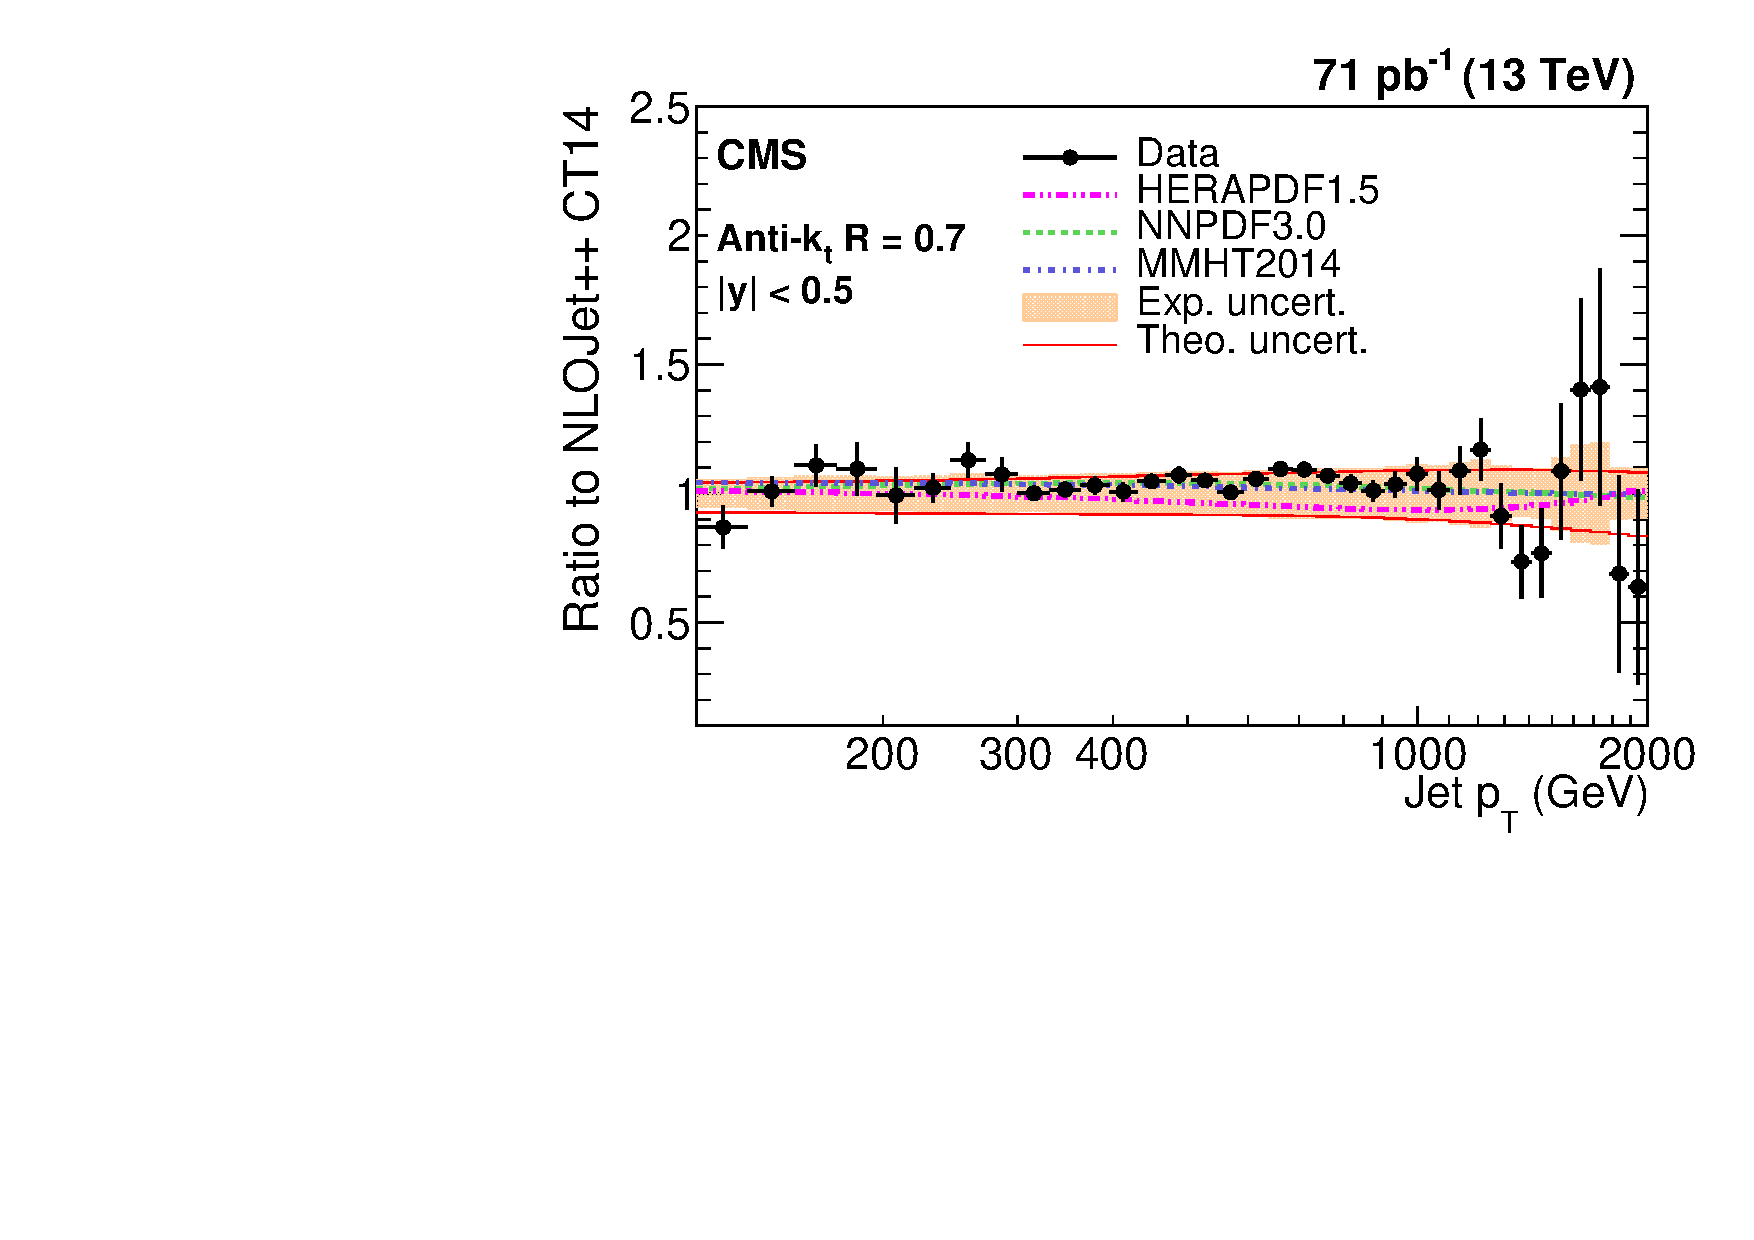
\includegraphics[width=0.48\textwidth]{Figure2-a.pdf}
  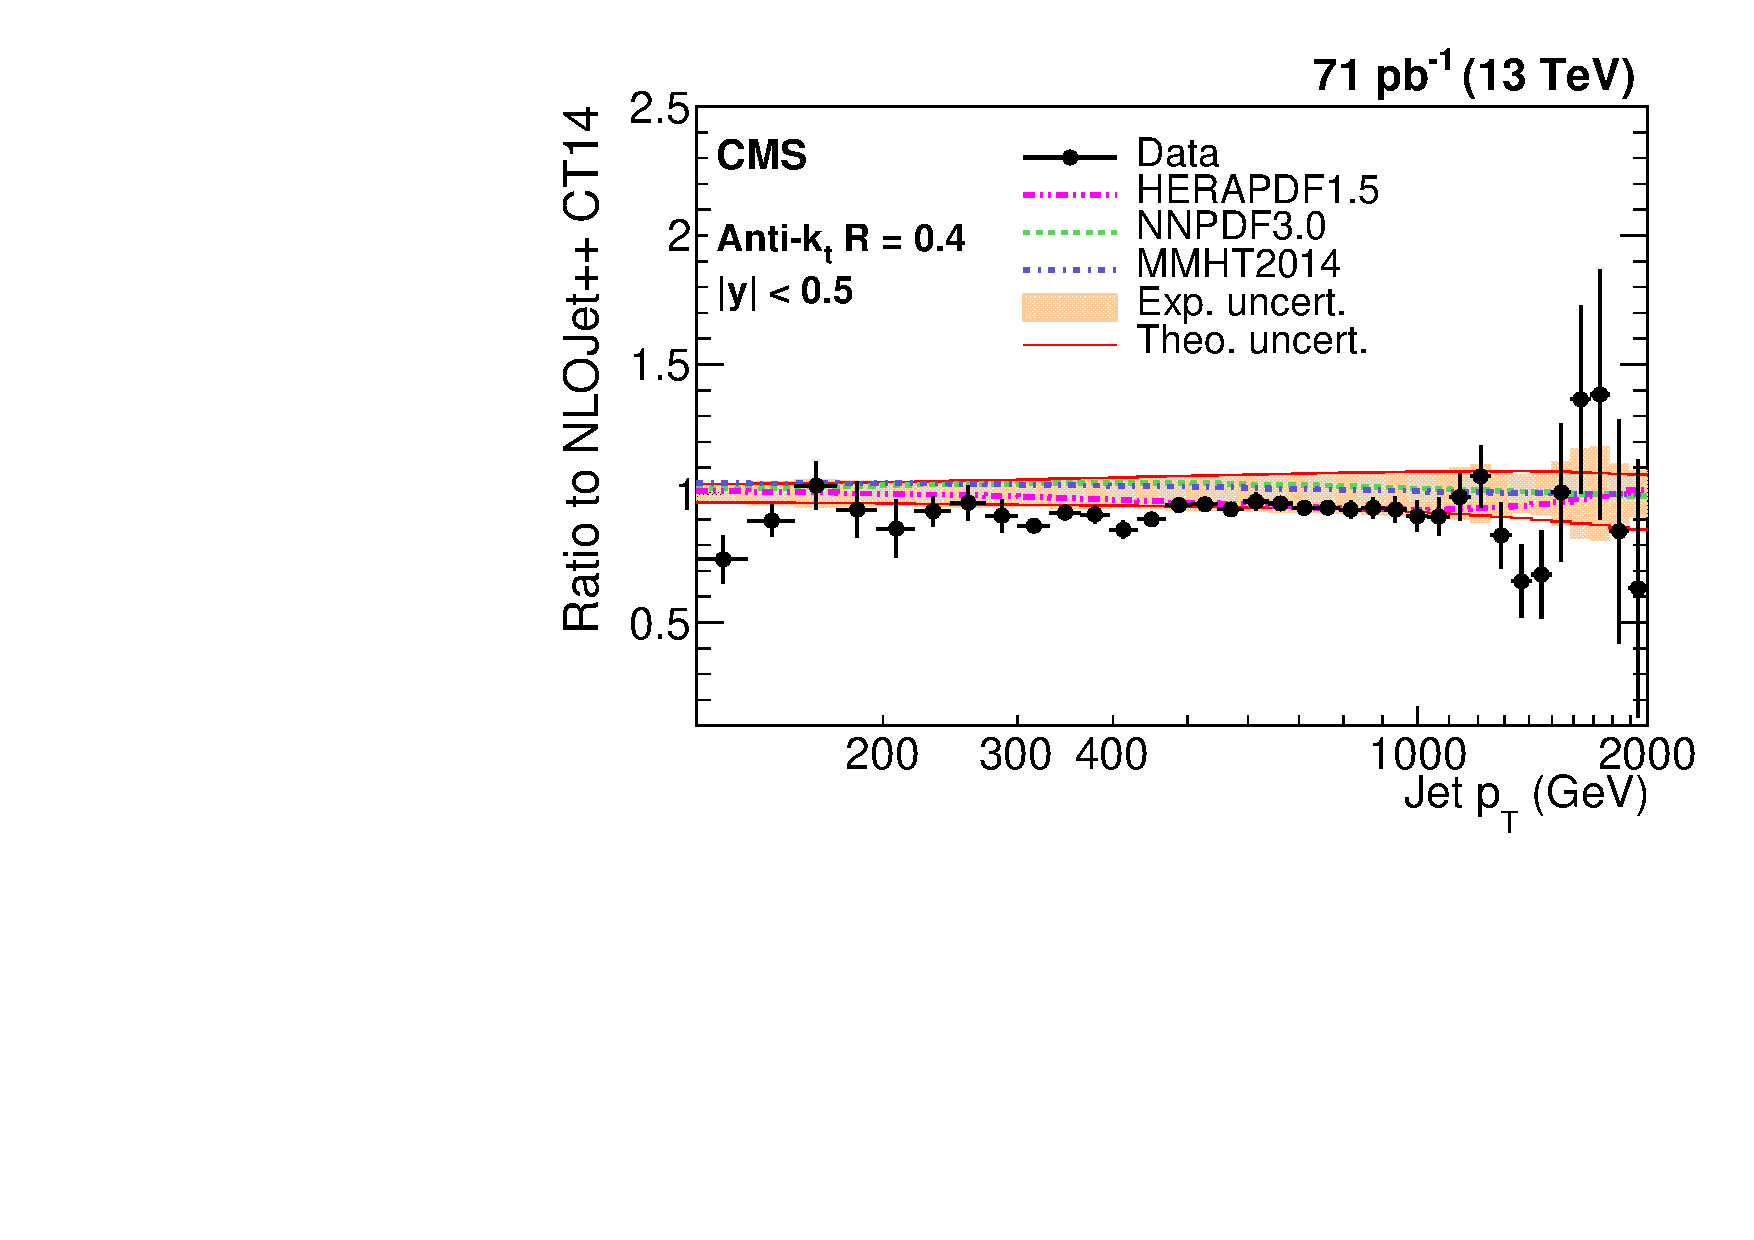
\includegraphics[width=0.48\textwidth]{Figure2-b.pdf}
  \caption{Ratio of measured values to theoretical prediction from \NLOJETPP using the CT14 PDF set and corrected for
the NP and electroweak effects. Predictions employing three other PDF sets are also shown for comparison. Jets are
clustered with the anti-\kts algorithm with a distance parameter of 0.7 and 0.4. The error bars correspond to the statistical
uncertainties of the data and the shaded bands to the total experimental systematic uncertainties.}
  \label{fig:ratio_CT14}
\end{figure*}

\section{Photon Physics}

\section{Conclusions}

\begin{thebibliography}{99}

\bibitem{Aad:2008zzm}
  G.~Aad {\it et al.} [ATLAS Collaboration],
  %``The ATLAS Experiment at the CERN Large Hadron Collider,''
  JINST {\bf 3} (2008) S08003.
  doi:10.1088/1748-0221/3/08/S08003

\bibitem{Chatrchyan:2008aa}
  S.~Chatrchyan {\it et al.} [CMS Collaboration],
  %``The CMS experiment at the CERN LHC,''
  JINST {\bf 3} (2008) S08004.
  doi:10.1088/1748-0221/3/08/S08004

\bibitem{Cacciari:2008gp}
  M.~Cacciari, G.~P.~Salam and G.~Soyez,
  %``The Anti-k(t) jet clustering algorithm,''
  JHEP {\bf 0804} (2008) 063
  doi:10.1088/1126-6708/2008/04/063
  [arXiv:0802.1189 [hep-ph]].
  %%CITATION = doi:10.1088/1126-6708/2008/04/063;%%
  %3828 citations counted in INSPIRE as of 15 Aug 2016

\bibitem{Lampl:2008zz} W.~Lampl {\it et al.}, %``Calorimeter clustering algorithms: Description and performance,''
ATL-LARG-PUB-2008-002, ATL-COM-LARG-2008-003.

\bibitem{CMS:2009nxa}
  [CMS Collaboration],
  %``Particle-Flow Event Reconstruction in CMS and Performance for Jets, Taus, and MET,''
  CMS-PAS-PFT-09-001.

\bibitem{Khachatryan:2016wdh} V.~Khachatryan {\it et al.} [CMS Collaboration], %``Measurement of the double-differential
inclusive jet cross section in proton-proton collisions at sqrt(s) = 13 TeV,'' [arXiv:1605.04436 [hep-ex]]. Submitted
to: Eur.Phys.J.C.

\bibitem{Nagy:2003tz}
  Z.~Nagy,
  %``Next-to-leading order calculation of three jet observables in hadron hadron collision,''
  Phys.\ Rev.\ D {\bf 68} (2003) 094002
  doi:10.1103/PhysRevD.68.094002
  [hep-ph/0307268].

\bibitem{Dulat:2015mca}
  S.~Dulat {\it et al.},
  %``New parton distribution functions from a global analysis of quantum chromodynamics,''
  Phys.\ Rev.\ D {\bf 93} (2016) no.3,  033006
  doi:10.1103/PhysRevD.93.033006
  [arXiv:1506.07443 [hep-ph]].



\end{thebibliography}

\end{document}
